\chapter{Medical Imaging}
\label{ch:rworks}

The imaging modalities used in biology and medicine are based on a variety of energy sources, including light, electrons, lasers, X-rays, radionuclides, ultrasound and nuclear magnetic resonance. The images produced span orders of magnitude in scale, ranging from molecules and cells to organ systems and the full body. The advantages and limitations of each imaging modality are primarily governed by the basic physical and biological principles which influence the way each energy form interacts with tissues, and by the specific engineering implementation for a particular medical or biological application.

\subsection{Modalities}
Each modality results from a different phenomenon of physics offers doctors (radiologists) an alternative view of the patient. Moreover each modality has it's risks, costs and benefits. All these factors have to be taken into account when choosing type of modality to be issued.

\subsubsection{X-Ray}
In 1895, Wilhelm Roentgen explored rays which could pass through wood and human tissues. He called them "x-rays" where "x" was considered as a place-holder for the unknown.

X-Rays are a form of electromagnetic radiation in the same spectrum as visible light and radio waves. Like light, x-rays can be considered as a energy of an x-ray photon. To make x-rays, it can be fired high-energy electrons into matter. In medical-imaging applications, x-rays are sent into tissue. 

Jointly x-rays interactions with matter it can be considered 3 common cases:
\begin{itemize}
    \item Photoelectric Effect
    \newline This effect is the principal effect that makes x-ray useful.
    \item Compton Interaction
    \newline Because of tissues tend to have little variations, Compton Interaction does not give precise information in terms of what is inside the body. 
    \item Rayleigh (Coherent) Scattering
    \newline Upon interacting with the attenuating medium, the photon does not have enough energy to liberate the electron from its bound state.
\end{itemize}

\subsubsection{Computed Tomography (CT)}
In simplified terms, the idea of computed tomography is to resolve a single slice of an object using many x-ray projections. As the gantry rotates, the scanner collects a 1D x-ray at each angle.

The CT scanners which designed for purpose of human diagnostic are generally capable of producing images with voxels, where voxel stand for representing a value on a regular grid in three-dimensional space    

The CT images which are span of x-rays are a form of ionizing radiation. Ionizing radiation is radiation with high enough energy that electrons can be ejected out of their orbitals, creating ions. These ions in large amounts can cause tissue and DNA damages. By this consideration medicine actively limits the amount of ionizing radiation the patient may potentially gets.

\item Contrast Agents
\newline
As the one of additional practices approaching CT for retrieving human body information, frequently substances can be introduced to the body to add the contrast, what is named as contrast agents. Often agents may be essentially useful for visualising of observations.          

\item Motion Artifacts
\newline
Usually it takes a few seconds to obtain one bit of CT data. The tidiness of the observations depends on whether the patient moved during the acquisition. If so, the resulting transformation will be inconsistent and the reconstructed image will contain errors. But, if the patient's motions are known, meaning a lot of artifacts can be corrected during the reconstruction. On top of it the few automatic methods can be applied to dare to sharpen the image by guessing the motions.

\subsubsection{Positron Emission Tomography (PET)}      
Similar to CT, PET approaches with ring of detectors to detect radiation. The raw data that comes out of a PET scanner is very similar in nature to the Radon transform in CT. Beyond, unlike CT scans PET ones take a long time to be acquired, meaning the patient motions can cause the problems. Moreover before issuing the measurements it is injected a small amount of positron-emitting radioisotope into the patient. This radioisotope is bound to a metabolite that is used glucose for instance.        

The list of images modalities and corresponding methods varies a lot strictly depending of the use case.
Below it is denoted few more popular directions:
\begin{itemize}
    \item MEG - Magneto Encephalography
    \item EEG - Electro Encephalography
    \item OCT - Optical Coherence Tomography
    \item SPECT - Single Photon Emission Computed Tomography
\end{itemize}


\subsection{Image Segmentation}
%ADD VISUALISATION
In terms of medical imaging, segmentation is the process of classifying pixels into groups which corresponds to the same tissue type. Segmentation has many uses cases like a "measure volume of an organ", "render a 3D view of an organ", "surface-based registration" and many others. Further we will descry types of segmentation. 

\subsubsection{Thresholding}
%ADD VISUALISATION 
The simplest method for classifying pixels based on solely on their intensity values. In thresholding we choose upper and lower bound and select pixels in predefined range.
The problem within simple thresholding is that it does not take into consideration any spatial information, meaning each pixel is evaluated no matter it locates.    

\subsubsection{Region Growing}
Unlike basic thresholding, region growing, which is iterative method, starts with the small set of seed pixels and grow out from them.
It's functionality can be easily represented within any basic draw editor. To do that we will draw empty grid rectangle and afterwards select interested region and apply function named flat fill color.  


\begin{figure}[h]
    \centering
    \subfloat[\centering Empty grid rectangle]{{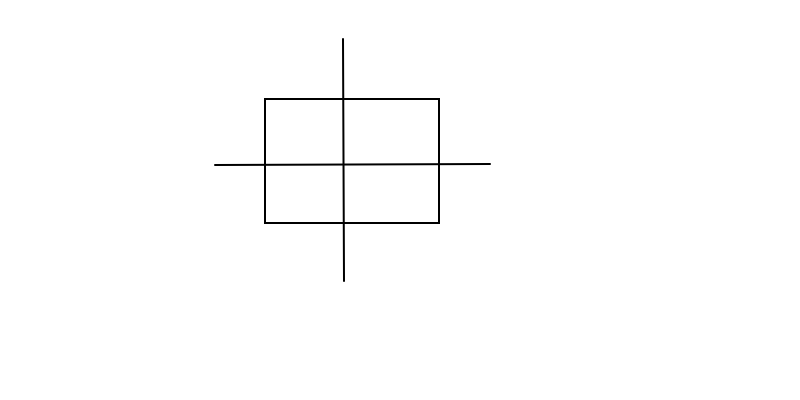
\includegraphics[width=5cm]{images/grow_region_0.png} }}%
    \qquad
    \subfloat[\centering Filled grid rectangle]{{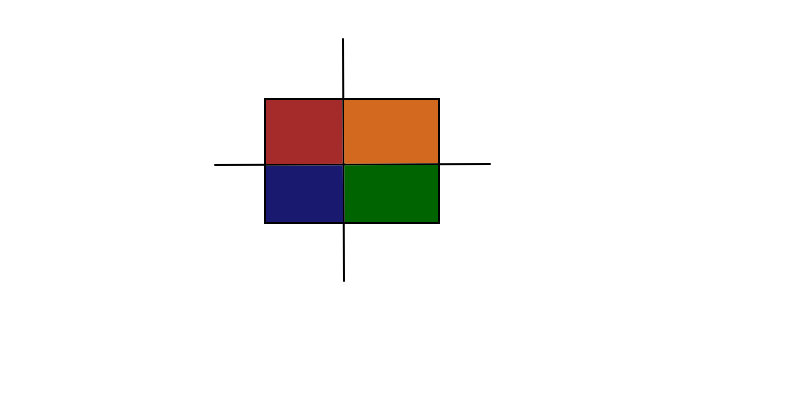
\includegraphics[width=5cm]{images/grow_region_1.png} }}%
    \caption{Region Growing Thresholding}%
    \label{fig:grwoing_region}%
\end{figure}



  
